\begin{table}[H]
  \caption{Нелинейные активационные функции}\label{actvs}
  \begin{tabular}{|c|c| c |}
    \hline    
    \hyperlink{name}{Название} & \hyperlink{func}{Функция} & \hyperlink{image}{Вид} \\
    \hline
    Сигмоидная & $\sigma(x)=\frac{1}{1+e^{-x}}$ & 
    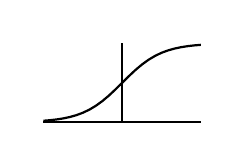
\begin{tikzpicture}[baseline={(0,0.5)},thick]
      \draw (-1,0) -- (1,0);
      \draw (0,0) -- (0,1);
      \path (-1.2,-0.2) rectangle (1.2,1.2);
      \draw plot[domain=-1:1,variable=\x] ({\x},{1/(1+exp(-4*\x))});      
    \end{tikzpicture} \\
    \hline
    Гиперболический тангенс &
    $\tanh(x)=\frac{e^x-e^{-x}}{e^z+e^{-z}}$
     & 
    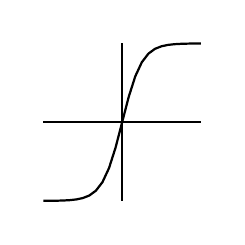
\begin{tikzpicture}[baseline={(0,0)},thick]
      \draw (-1,0) -- (1,0);
      \draw (0,-1) -- (0,1);
      \path (-1.2,-1.2) rectangle (1.2,1.2);
      \draw plot[domain=-1:1,variable=\x] ({\x},{tanh(4*\x)});
    \end{tikzpicture} \\
    \hline
    ReLU & $f(x) =\begin{cases}
    0 & ~\text{if}~ x<0 \\ 
    x & ~\text{if}~x \geq 0.
    \end{cases}$ & 
    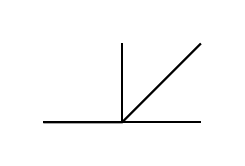
\begin{tikzpicture}[baseline={(0,0.5)},thick]
      \draw (-1,0) -- (1,0);
      \draw (0,0) -- (0,1);
      \path (-1.2,-0.2) rectangle (1.2,1.2);
      \draw plot[domain=-1:1,variable=\x] ({\x},{ifthenelse(\x<0,0,\x)});
    \end{tikzpicture}\\          
    \hline            
  \end{tabular}
\end{table}